\documentclass{standalone}

\usepackage{libertinus}
\usepackage[T1]{fontenc}
\renewcommand*\familydefault{\sfdefault}

\usepackage{DejaVuSansMono}

\usepackage{tikz}
\tikzset{every path/.style={semithick}}

\begin{document}
  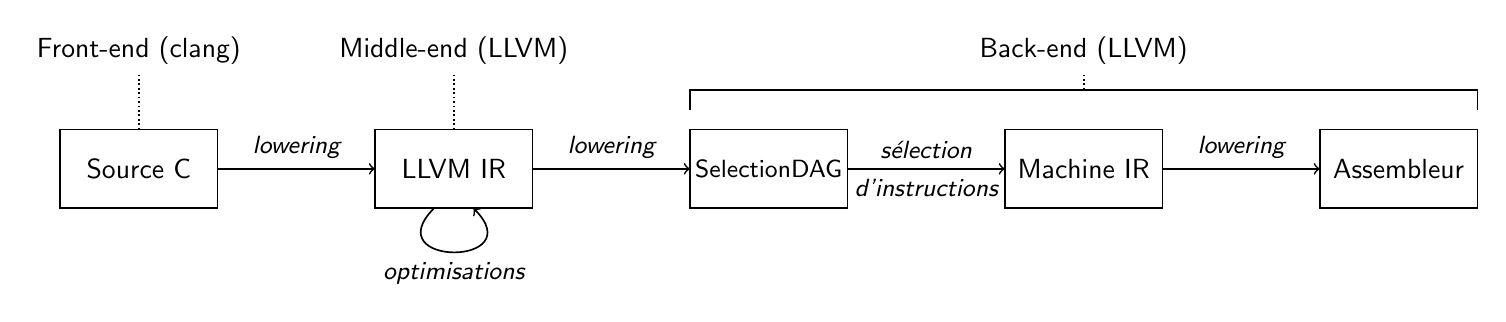
\begin{tikzpicture}
    \draw (0,0) rectangle node {Source C} ++(2,1);
    \draw (4,0) rectangle node {LLVM IR} ++(2,1);
    \draw (8,0) rectangle node {\small SelectionDAG} ++(2,1);
    \draw (12,0) rectangle node {Machine IR} ++(2,1);
    \draw (16,0) rectangle node {Assembleur} ++(2,1);

    \node (FE) at (1,2) {Front-end (clang)};
    \node (ME) at (5,2) {Middle-end (LLVM)};
    \node (BE) at (13,2) {Back-end (LLVM)};

    \draw[densely dotted] (FE) -- (1,1);
    \draw[densely dotted] (ME) -- (5,1);
    \draw[densely dotted] (BE) -- (13,1.5);
    \draw (8,1.25) |- ++(10,0.25) -- ++(0,-0.25);

    \draw[->] (2,0.5) -- node[above] {\small\it lowering} ++(2,0);
    \draw[->] (6,0.5) -- node[above] {\small\it lowering} ++(2,0);
    \draw[->] (10,0.5) -- node[above] {\small\it sélection} node[below] {\small\it d'instructions} ++(2,0);
    \draw[->] (14,0.5) -- node[above] {\small\it lowering} ++(2,0);

    \draw[->] (4.75,0) to[out=225, in=315, distance=30] node[below] {\small\it optimisations} (5.25,0);
  \end{tikzpicture}
\end{document}
